\documentclass[12pt,spanish]{report}
\usepackage[spanish,mexico]{babel}
\usepackage[utf8]{inputenc}
\usepackage[rightcaption]{sidecap}
\usepackage{wrapfig}
\usepackage{graphicx} %package to manage images
\graphicspath{ {Pictures/} }
\usepackage{amsmath}
\usepackage{amsthm}
\usepackage{dsfont}
\usepackage{amsfonts}
\usepackage{amssymb}
\usepackage{mathrsfs}
\usepackage{mathtools}
\usepackage{enumerate} %% Sirve para poder usar entornos como \itemize, \list_type, \enumerate, ...
\usepackage{float} %%Para poner las figuras donde se desea
\usepackage{url} %%Para agregar páginas de internet
\usepackage{makeidx}
\usepackage{verbatim} %% Para poder agregar textos tal cual se escriben, por ejemplo los códigos sin que se modifiquen.
%\setlength{\parindent}{0mm} %% Los párrafos NO tienen sangría
\usepackage{hyperref} %%Sirve para hacer referencias dentro del texto, por ejemplo para un libro en la Bibliografía o un ecuación necesaria. %% También se debe compilar 2 veces con PDFLATEX, ya que en la 1° guarda la información de la numeración de las ecuaciones y en la 2° escribe esa información en el documento.
\usepackage{multirow} %% Para tener tablas con varios renglones
\usepackage{adjustbox}


%%Definición de variables
\newcommand{\dfNmatrizChica}{\begin{table}[H]
\centering
\resizebox{\textwidth}{!}{%
\begin{tabular}{|c|l|p{7cm}|p{3.5cm}|}
\hline
Col. & Nombre      & Explicación                                           & Posibles                       \\ \hline
1     & Semestre    & Semestre al que pertenece la materia (Año y semestre) & $1^{o}, 2^{o},..., 8^{o}$      \\ \hline
2     & Plan        & Año en el que se implemento un nuevo plan de estudios & Número de plan de estudios     \\ \hline
3     & Materia     & Clave del curso impartido                             & $\mathbb{N}$                   \\ \hline
4     & URL         & Nombres de las páginas de los horarios de FC          & Nombres de páginas de internet \\ \hline
5     & Num. Grupos & Número de grupos que hay en cada página de internet   & $\mathbb{N}$                   \\ \hline
\end{tabular}%
}
\end{table}}

\newcommand{\dfNmatrizGrande}{\begin{table}[H]
\centering
\resizebox{\textwidth}{!}{%
\begin{tabular}{|c|l|p{7cm}|p{3.5cm}|}
\hline 
Col. & Nombre & Explicación & Posibles valores \\ 
\hline 
1 & Materia & Nombre del curso impartido & Nombres de materias \\ 
\hline 
2 & Profesor & Nombre de la persona que va a impartir alguna materia & Nombres de personas \\ 
\hline 
3 & Horario & Hora en la que se imparte alguna materia & 15 horas en total \\ 
\hline 
4 & Lugares & Espacios disponibles por salón & $\mathbb{N}$ \\ 
\hline 
5 & Alumnos & Número de estudiantes inscritos por grupo & $\mathbb{N}$ \\ 
\hline 
6 & Salón & Espacio físico en el que se imparte alguna materia & Nombres de salones \\ 
\hline 
7 & Grupo & Clave con la que se identifica una asignación & Clave de grupos \\ 
\hline 
%8 & Carrera & Nombre de alguna carrera de FC & Actuaría, Ciencias de la Computación, Matemáticas, Matemáticas Aplicadas \\ 
8 & Carrera & Nombre de alguna carrera de FC & Actuaría, C. de la C., Mate, Mate Ap. \\ 
\hline 
9 & Plan & Año en el que se implemento un nuevo plan de estudios & Número de plan de estudios \\ 
\hline 
10 & Semestre & Semestre al que pertenece la materia (Año y semestre) & $1^{o}, 2^{o},..., 8^{o}$ \\ 
\hline 
11 & Cambios & Clave que indica los cambios que se le han hecho al grupo & $1,2,3$ \\ 
\hline 
12 & Turno & Matutino: 7:00-14:00hrs, Vespertino: 15:00-21:00 & Matutino/Vespertino \\ 
\hline 
13 & Sem.Materia & Semestre en el que el plan de estudios dicta que se lleva esa materia & ``Primer'', ``Segundo'', $\ldots$ ``Octavo'', ``Optativas'' \\ 
\hline 
\end{tabular}%
}
\end{table}}



\begin{document}

\begin{center}
\textbf{Limpieza de Base}
\end{center}

\begin{itemize}

\item[-] Sólo se tomará en cuenta la información de las carreras del Departamento de Matemáticas, es decir, Actuaría, Matemáticas, Matemáticas Aplicadas y Ciencias de la computación.

\item[-] Para encontrar los horarios de cada materia se observó que la estructura que se sigue es la siguiente:

\begin{center}
``http://www.fciencias.unam.mx/docencia/horarios/a/b/c''
\end{center}

De esta manera se hicieron 3 ciclos de tipo ``for'', inicialmente los valores de $a, b $ y $c$ eran:

$a$: 20081, 20082, 20091, 20092, 20101, 20102, $\ldots,$ 20201

$b: 1:10000$

$c: 1:10000$

\item[-] Se buscó un patrón en las páginas para disminuir el número de combinaciones por lo que los valores que se encontraron fueron: a = semestre, b = plan de estudios, c = número de materia, por lo que los ciclos corren:

Semestre: 20081, 20082, 20091, 20092, 20101, 20102, $\ldots,$ 20201

Plan: Planes de estudio

Núm. Materia: $1:10000$

Los planes de estudio de cada carrera son:

\begin{itemize}
\item[*] Actuaría:

1972 $\rightarrow$ plan = 214

2000 $\rightarrow$ plan = 119

2006 $\rightarrow$ plan = 1176

2015 $\rightarrow$ plan = 2017

Los planes vigentes son los últimos tres.

\item[*] Ciencias de la Computación:

1994 $\rightarrow$ plan = 218

2013 $\rightarrow$ plan = 1556

\item[*] Matemáticas:

1983 $\rightarrow$ plan = 217

\item[*] Matemáticas Aplicadas:

2017 $\rightarrow$ plan = 2055
\end{itemize}


\begin{table}[H]
\centering
\begin{tabular}{|c|c|}
 \hline 
  PLAN & CLAVE \\ 
 \hline 
 \multicolumn{2}{|c|}{Actuaría} \\ 
 \hline 
 1972 & 214 \\ 
 \hline 
 2000 & 119 \\ 
 \hline 
 2006 & 1176 \\ 
 \hline 
 2015 & 2017 \\ 
 \hline 
 \multicolumn{2}{|c|}{Ciencias de la Computación} \\ 
 \hline 
 1994 & 218 \\ 
 \hline 
 2013 & 1556 \\ 
 \hline 
 \multicolumn{2}{|c|}{Matemáticas} \\ 
 \hline 
 1983 & 217 \\ 
 \hline 
 \multicolumn{2}{|c|}{Matemáticas Aplicadas} \\ 
 \hline 
 2017 & 2055 \\ 
 \hline 
 \end{tabular}  
%\caption{\textit{a}}
\end{table}



\item[-] Al inicio se encontraron tres tipos de grupos de las páginas de horarios de la FC:

\begin{enumerate}
\item[a)] Las páginas correspondientes al semestre $2020-1$, la cual no contiene la información de los exámenes finales. \url{http://www.fciencias.unam.mx/docencia/horarios/20201/2017/1707}

\begin{figure}[H]
\centering
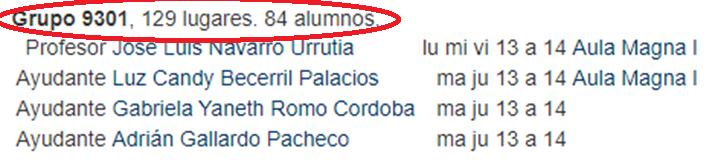
\includegraphics[scale = 0.45]{GrupoA} %width=\textwidth
%\caption{\textit{a}}
\end{figure}


\item[b)] Páginas correspondientes a semestres entre el $2018-2$ y el semestre $2019-2$, las cuales tienen información del número de lugares disponibles por salón. \url{http://www.fciencias.unam.mx/docencia/horarios/20182/217/625}

\begin{figure}[H]
\centering
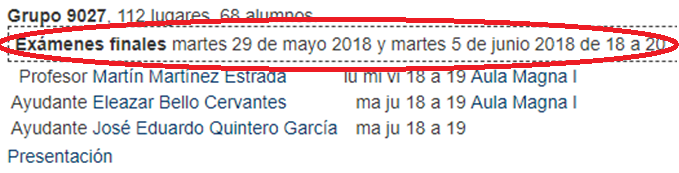
\includegraphics[scale = 0.45]{GrupoB} %width=\textwidth
%\caption{\textit{a}}
\end{figure}

\item[c)] Páginas correspondientes a semestres anteriores al $2018-1$, incluyéndolo, éstas páginas no contienen la información del número de lugares disponibles por cada salón. \url{http://www.fciencias.unam.mx/docencia/horarios/20181/1556/399}
\end{enumerate}

\begin{figure}[H]
\centering
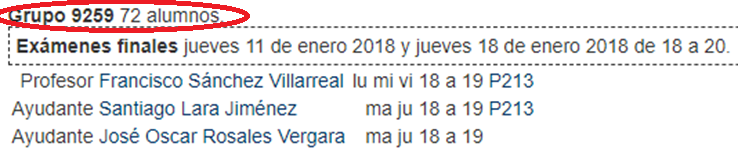
\includegraphics[scale = 0.45]{GrupoC} %width=\textwidth
%\caption{\textit{a}}
\end{figure}

\item[-] Al querer obtener la información de las páginas de la matriz, se encontraron otros tipos de página:

\begin{enumerate}
\item[4.] Páginas en las cuales se tiene el nombre de la materia, pero no hay información de algún grupo, por ejemplo \url{http://www.fciencias.unam.mx/docencia/horarios/20081/1556/803}

\begin{figure}[H]
\centering
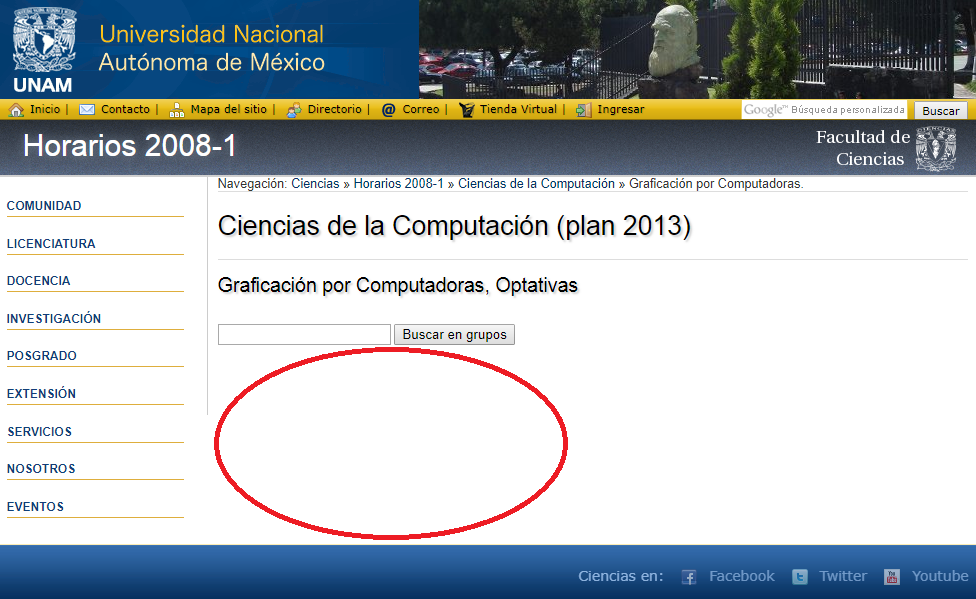
\includegraphics[scale = 0.45]{FaltaInfo_A} %width=\textwidth
%\caption{\textit{a}}
\end{figure}

\item[5.] Páginas que no tienen información del salón: \url{http://www.fciencias.unam.mx/docencia/horarios/20081/119/4}

\begin{figure}[H]
\centering
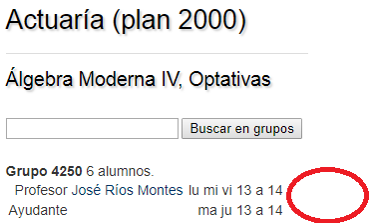
\includegraphics[scale = 0.45]{FaltaInfo_B} %width=\textwidth
%\caption{\textit{a}}
\end{figure}

\item[6.] Páginas que tienen grupos sin información del número de alumnos: \url{http://www.fciencias.unam.mx/docencia/horarios/20112/119/630}

\begin{figure}[H]
\centering
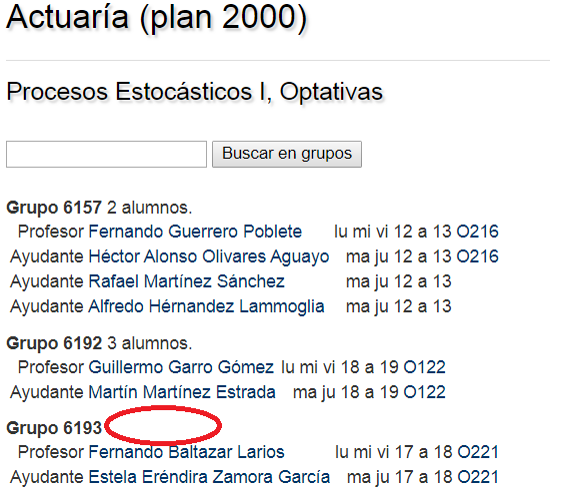
\includegraphics[scale = 0.45]{FaltaInfo_C} %width=\textwidth
%\caption{\textit{a}}
\end{figure}

\item[7.] Páginas que tienen grupos sólo con el horario (sin nombre del profesor, salón, ayudante, número de alumnos, lugares disponibles): \url{http://www.fciencias.unam.mx/docencia/horarios/20091/119/841} \url{http://www.fciencias.unam.mx/docencia/horarios/20091/119/244}

\begin{figure}[H]
\centering
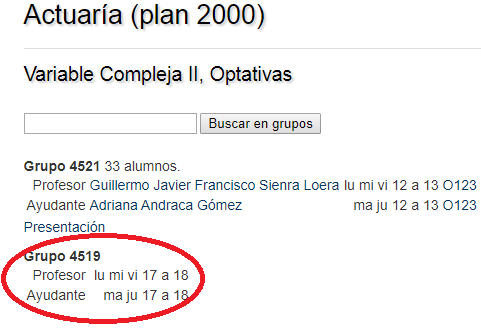
\includegraphics[scale = 0.6]{FaltaInfo_D} %width=\textwidth
%\caption{\textit{a}}
\end{figure}


\end{enumerate}


\item[-] Una vez que se probó la función \verb+posibles_url+ se obtuvo una primera matriz llamada \verb+mat_posibles_url+, con $18 725$ entradas, ahí se observó que el número máximo de materia es 991, por lo que el valor máximo se puede reducir de $10 000$ a $1 000$.

\item[-] La matriz \verb+mat_posibles_url+ se define con un tamaño fijo antes de correr el algoritmo para que no se demore por tener un objeto que va cambiando de tamaño, por lo que al final de haberle aplicado la función se le deben de quitar los renglones que no tienen información.

\item[-] Dentro de los problemas de información repetida, se encontraron 2 posibles casos:

\begin{enumerate}
\item Tener información de una materia correspondiente a un plan de estudios posterior al semestre: \url{http://www.fciencias.unam.mx/docencia/horarios/20082/1556/803} y tener la misma información con el plan de estudios correspondiente: \url{http://www.fciencias.unam.mx/docencia/horarios/20082/218/803}

\begin{figure}[H]
\centering
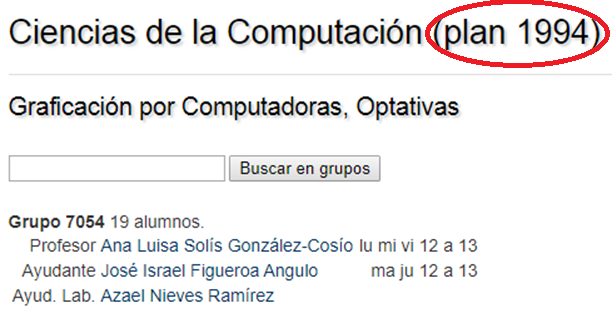
\includegraphics[scale = 0.45]{InfoRepetida_A_1} %width=\textwidth
%\caption{\textit{a}}
\end{figure}

\begin{figure}[H]
\centering
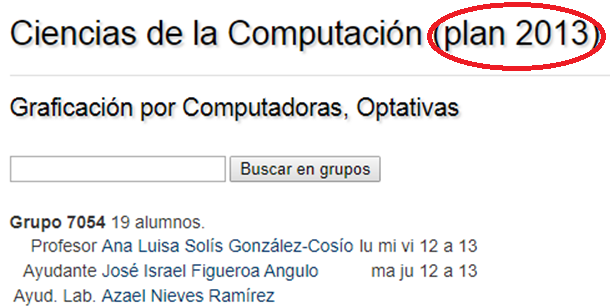
\includegraphics[scale = 0.45]{InfoRepetida_A_2} %width=\textwidth
%\caption{\textit{a}}
\end{figure}

\item Tener una misma materia con nombres distintos para las diferentes carreras: \url{http://www.fciencias.unam.mx/docencia/horarios/20201/2017/1739} para Actuaría, plan 2015 y \url{http://www.fciencias.unam.mx/docencia/horarios/20201/217/1712} para Matemáicas, plan 1983. Notamos que la información en ambas páginas es la misma, sólo se cambia el orden en la que se encuentran los grupos.
\end{enumerate}

\begin{figure}[H]
\centering
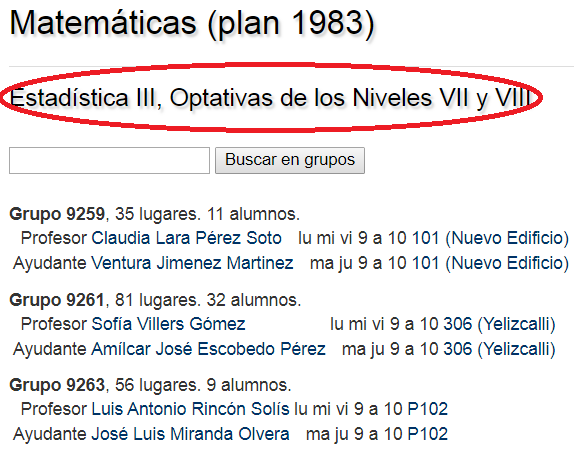
\includegraphics[scale = 0.45]{InfoRepetida_B_1} %width=\textwidth
%\caption{\textit{a}}
\end{figure}

\begin{figure}[H]
\centering
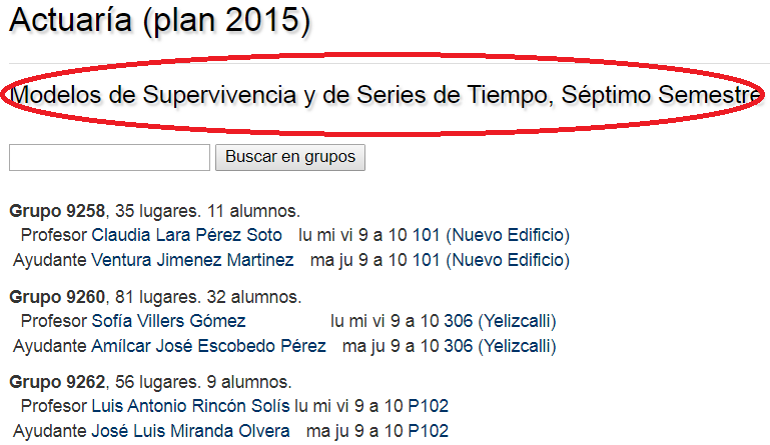
\includegraphics[scale = 0.45]{InfoRepetida_B_2} %width=\textwidth
%\caption{\textit{a}}
\end{figure}


\item[-] En la función \verb+genera_m13+ se obtiene una matriz con 13 columnas: Materia, Profesor, Horario, Lugares, Alumnos, Salón, Grupo, Carrera, Plan, Semestre, Cambios, Turno, Sem. Materia.

La columna 11, \textit{Cambios}, va a guardar todos los cambios que han ``sobrevivido'' esas páginas, dependiendo los números que se encuentren serán los cambios de cada url.

\begin{enumerate}
\item[(1)] Corresponde a que se eliminaron las copias de los planes de estudio viejos

\item[(2)] Corresponde a que se eliminaron las copias de las materias que tienen nombres distintos para carreras diferentes

\item[(3)] Corresponde a las páginas que no tienen información del salón
\end{enumerate}

La columna 12, \textit{Turno}, va a ser una columna binaria en la cual habrá un $1$ si el turno es matutino el cual consideraremos que será desde las $7am$ hasta las $2pm$, tomando en cuenta la clase que comienza a las $2pm$ y termina a las $3pm$; y habrá un $0$ si el turno es vespertino, considerado de $3pm$ a $9pm$, contando como clase inicial la de $3-4pm$ y como la última clase la de $9-10pm$


La columna 13, \textit{Sem. Materia}, contiene el semestre en el que el plan de estudios dicta que se lleva esa materia. Ej. ``Primer'', ``Segundo'', $\ldots$ ``Octavo'', ``Optativas''

\item[-] Las categorías de las columnas de $m5$ son:

\dfNmatrizChica %%Tabla con la información de la matriz chica

\begin{figure}[H]
\centering
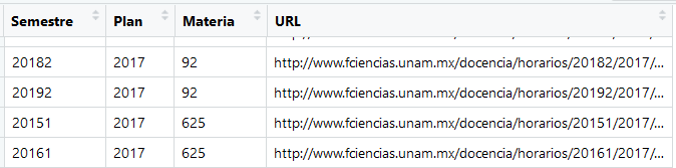
\includegraphics[scale = 0.45]{m4} %width=\textwidth
%\caption{\textit{a}}
\end{figure}


\item[-] Las categorías de las columnas de $m13$ son:

\dfNmatrizGrande %%Tabla con la información de la matriz grande



%\begin{figure}[H]
%\centering
%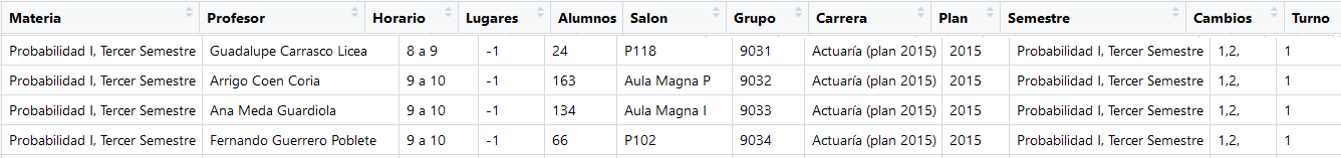
\includegraphics[scale = 0.4]{m12} %width=\textwidth
%%\caption{\textit{a}}
%\end{figure}


\item[-] Se obtuvieron $4$ grupos de datos para hacer los análisis estadísticos:

\begin{itemize}
\item[$G_{1}:$] Turno matutino semestre impar

\item[$G_{2}:$] Turno vespertino semestre impar

\item[$G_{3}:$] Turno matutino semestre par

\item[$G_{4}:$] Turno vespertino semestre par
\end{itemize}

\begin{table}[H]
\centering
\begin{tabular}{|c|c|c|}
\hline 
Sem. $\setminus$ Turno & Matutino & Vespertino \\ 
\hline 
Impar & $G_{1}$ & $G_{2}$ \\ 
\hline 
Par & $G_{3}$ & $G_{4}$ \\ 
\hline 
\end{tabular} 
%\caption{\textit{a}}
\end{table}


\item[-] Problemas con la extracción de información en las páginas web
\begin{enumerate}
\item Dentro de la obtención de datos del número de alumnos, no se lee la información cuando se tiene \textit{Un alumno}
\end{enumerate}

\end{itemize}

\end{document}
